\documentclass[12pt]{report}
\usepackage[pdftex]{graphicx}
\newcommand{\HRule}{\rule{\linewidth}{0.5mm}}
% correct bad hyphenation here
\hyphenation{op-tical net-works semi-conduc-tor auto-nomous}


\begin{document}
%
% paper title
% can use linebreaks \\ within to get better formatting as desired
\title{Design of an Attitude and Heading Reference Sensor}
\author{Patrick Hickey\\pat@moreproductive.org}
\begin{titlepage}
\begin{center}

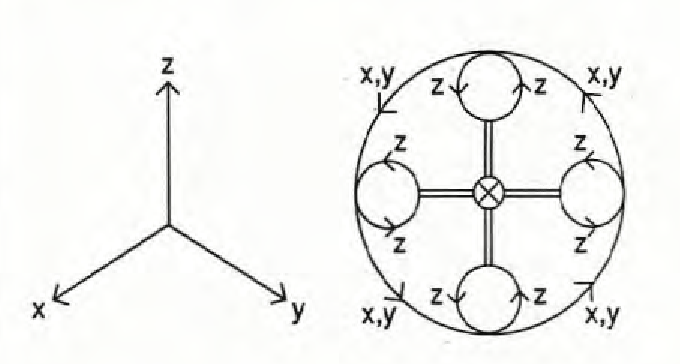
\includegraphics[width=0.3\textwidth]{./cycloid.png}\\[2cm]
\HRule \\[1cm]
{ \huge \bfseries Design of an Attitude and Heading Reference Sensor } \\[1cm]
\HRule \\[0.5cm]
{ \large \bfseries Presented for completion of an Independent Study in Electrical Engineering }
\\[0.5cm]
{ \large \bfseries Rutgers, The State University of New Jersey }
\\[0.5cm]
\HRule \\[1cm]

{\large Pat Hickey}
\\ 
pat@moreproductive.org
\\[0.5cm]
\emph{Advisor}
\\ Dr. Chung-chieh Shan
\\ Department of Computer Science
\vfill
{\large \today}

\end{center}
\end{titlepage}


\begin{abstract}
This paper describes the design of an Attitude and Heading Reference Sensor (AHRS), which measures rootational orientation relative to north and down. 
The design uses 3-axis accellerometer, magnetometer, and rate gyro sensors. 
I will discuss the selection and construction of the sensor hardware, design and implementation of a Kalman filter for sensor fusion, and the test of both the sensor hardware and software.
\end{abstract}


\section{Problem Description}
Problem Statement
\subsection{Application}
aircraft autopilot
- in particular, paparazzi for linux
- soft real-time
- threads, c, linux
\subsection{Use of Haskell}
It is well established how to implement such a filter in C

I approached using a functional language as an experiment

\section{Hardware}
\subsection{Sensors}
needed 3 axis magnetometer, accellerometer, rate gyro
selected two ics:
invensense itg3200
st micro ...
\subsection{Microcontroller}
uart required to talk to a pc (ttyUSB), i2c required to talk to sensors
arduino pro mini was a simple solution, easy to use programming environment
\subsection{Construction}
provide photographs, schematic


\section{Embedded Software}
\subsection{Requirments}
timing and communication requirments of embedded hardware
st acc self test
\subsection{Communication Protocol}
serial strings etc.
\subsection{Arduino Environment}
describe arduino programming environment
blocking serial calls
-- Provide timing information?

\section{Filtration Software}
The filtration software was implemented in Haskell. The code may be found on Github at http://github.com/pchickey/hs-qkf/
\subsection{Algorithm Selection}
find an algorithm which assumes my measurment sources
\subsection{Algorithm Overview}
maybe a flow diagram would help here
\subsection{Implementation of Filter}
hmatrix-static
quaternions
\subsection{Implementation of Tests}
euler models
rotation-matrix based vector measurment simulation
addition of noise
\subsection{Sensor Interface}
serial.hs
\subsection{Gnuplot Interface}
overview, code snippets
\subsection{OpenGL Demonstration Interface}
cube.hs overview, code snippets 
\subsection{Paparazzi Autopilot Interface}
ffi, linux mq
"ongoing investigation"

\section{Results}
\subsection{Noise-free simulated measurments}
Plots of step test, ramp test
\subsection{Noisy simulated measurments}
step test, ramp test
\subsection{Tests with Sensor}
plots, link to video on youtube

\end{document}


